\documentclass{article}
\usepackage{arxiv}
\usepackage[utf8]{inputenc} % allow utf-8 input
\usepackage[T1]{fontenc}    % use 8-bit T1 fonts
\usepackage{hyperref}       % hyperlinks
\usepackage{url}            % simple URL typesetting
\usepackage{booktabs}       % professional-quality tables
\usepackage{amsfonts}       % blackboard math symbols
\usepackage{nicefrac}       % compact symbols for 1/2, etc.
\usepackage{microtype}      % microtypography
\usepackage{lipsum}
\usepackage{float}
\usepackage{graphicx}
\usepackage{listings}
\usepackage{xcolor}
\usepackage{amssymb,amsmath}
\usepackage{parskip}
\usepackage{fancyhdr}
\usepackage{tabu}
\usepackage{enumerate}
\usepackage{xcolor}
\usepackage{mathtools}
\usepackage{hyperref}
\usepackage{color}
\usepackage{pdfpages}
\definecolor{dkgreen}{rgb}{0,0.6,0}
\definecolor{gray}{rgb}{0.5,0.5,0.5}
\definecolor{mauve}{rgb}{0.58,0,0.82}

\lstset{frame=tb,
  language=Python,
  aboveskip=3mm,
  belowskip=3mm,
  showstringspaces=false,
  columns=flexible,
  basicstyle={\small\ttfamily},
  numbers=none,
  numberstyle=\tiny\color{gray},
  keywordstyle=\color{blue},
  commentstyle=\color{dkgreen},
  stringstyle=\color{mauve},
  breaklines=true,
  breakatwhitespace=true,
  tabsize=3
}
\hypersetup{
    colorlinks=true,
    linkcolor=blue,
    filecolor=magenta,      
    urlcolor=cyan,
    pdftitle={Sharelatex Example},
    bookmarks=true,
    pdfpagemode=FullScreen,
    }
%%%%%%%%%%%%%%%%S Some Macros %%%%%%%%%%%%%%%%%%%


\DeclarePairedDelimiter\ceil{\lceil}{\rceil}
\DeclarePairedDelimiter\floor{\lfloor}{\rfloor}
\newcommand{\qed}{\hfill $\blacksquare$}      




\title{TRAJECTORY PLANNING FOR MOBILE ROBOTS}


\author{
  Dinesh Jagai \\
  Department of Computer Science\\
 University of Pennsylvania \\
 Philadelphia, PA \\  
  \texttt{dinesh97@seas.upenn.edu} \\
  %% examples of more authors
  \And
  Thomas Wang \\
  Department of Computer Science\\
 University of Pennsylvania \\
 Philadelphia, PA \\  
  \texttt{ttwang@seas.upenn.edu} \\

  %% \AND
  %% Coauthor \\
  %% Affiliation \\
  %% Address \\
  %% \texttt{email} \\
  %% \And
  %% Coauthor \\
  %% Affiliation \\
  %% Address \\
  %% \texttt{email} \\
  %% \And
  %% Coauthor \\
  %% Affiliation \\
  %% Address \\
  %% \texttt{email} \\
}

\begin{document}
\maketitle
\section{Overview}
\section{Concepts}
\begin{enumerate}
    \item I'm going to implement A* algorithm because it's seems intuitive and similar to Dijkstra algorithm. The strategy here is to find the shortest path to the goal while considering the Euclidean distance to the goal. I plan in the configuration space.
        
    \item A* algorithm will check each time if the next step is blocked by an obstacle. If the step is blocked, the algorithm won't take that step, and will consider the others around it. To detect collision, we can check if the next step is in the middle of any obstacle by checking the coordinates, and invalid steps are those that have coordinates inside an obstacle's space. 
    
    Trajectory generating strategy: 
    The code for the trajectory is shown in listing-2 
    The bulk of the code is in the update function. The trajectory strategy is essentially to follow the way-points using linear paths - namely $x \And y$ lines. In order for the robot to face the consecutive way points, it's turns/circle's in place.
    Since we need a really tight circle, we assume that there are no limits on turning radius. \\ 
    In a dynamic situation my trajectory might not converge to the destination. Firstly, it takes a while to turn move to move to each consecutive waypoint. Also, in a vastly changing environment, it can get the robot can get confused when turning between the way-points. \\ 
    
    
        
    \item \textbf{Pseudocode for the planner} \\ 
    Start from the starting location by creating a Node there. Each Node contains their coordinate, their parent node, and their g, h, f values. Initialize a heapq for the ordering of nodes to visit based on their f value. The node with smallest f would be the first node. First put start node into the heapq. While the queue isn't empty, we will explore the map. At each loop, we will pop the first thing off the heapq, which has the smallest f value. For this node, we will explore the 8 nodes around it. For each of the 8 nodes around it, we will first check if it's within bounds and if it's collided with an obstacle. Add all of these nodes in a list called children. For each of the children, we will calculate their g, h, f values and record the parent. Then, add these children nodes into the heapq. The loop goes on, until the current node is the goal node. When it arrives at the goal node, follow the parents all the way back to the start node, and create an array. Reverse this array, and return this path.
 
         
\end{enumerate}         
\newpage

\section{Coding Assignment}

\lstinputlisting[caption = Astar.py]{Astar-3.py}

The idea of the algorithm is here and it works for a lot of the maps and routes, but we did encounter a few bugs along the way. For example, since the step size was set as 0.5, if there are gaps that are less than 0.5, this algorithm wouldn't be able to find that path. Also, there isn't a 'max iteration' set, so in some cases it might take a long time to output None.
\newpage

\lstinputlisting[caption = mobile\_path.py]{mobile_path.py}
The trajectory code and strategy mentions the one talked about in section 2. That is, a trajectory that consists of linear paths between the point and rotates to face consecutive waypoints.

All other modified code is included in the appendix. \\ 

\newpage

\section{Simulation}

\section{Questions To Think About} 

\begin{enumerate}
    \item The A* and RRT successfully found the path every time.
    
    \item A* takes about 0.5 seconds, but RRT can take very different times. Going across map1, one time it took 3 seconds and a different time it took 49 seconds.
    
    \item A* has the same path every time, but RRT has different paths each time.
    
    \item  The following maps are for A*
    For map 1 
    The time for planning for world 1 was 7.66 seconds  and the trajectory is inserted below: \\ 
    \renewcommand{\thefigure}{5.1.4.1}
\begin{center}
    \begin{figure}[H]
        \centering
        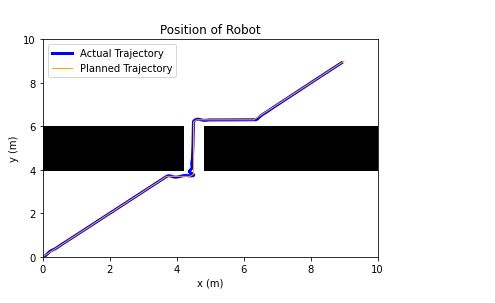
\includegraphics[width=18cm]{w1.JPG}
         \caption{Figure Showing path planning for world 1}
    \end{figure}
\end{center}

    The time for planning for world 2 was 4.97 seconds  and the trajectory is inserted below: \\ 
    \renewcommand{\thefigure}{5.1.4.2}
\begin{center}
    \begin{figure}[H]
        \centering
        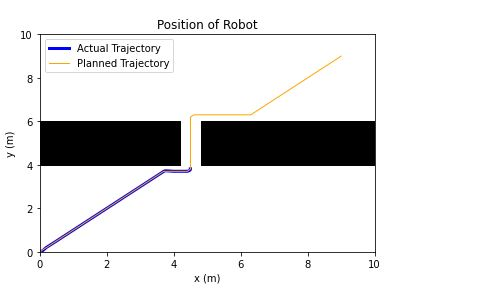
\includegraphics[width=18cm]{w2.JPG}
         \caption{Figure Showing path planning for world 2}
    \end{figure}
\end{center}

    The time for planning for world 3 was 7.6 seconds  and the trajectory is inserted below: \\ 
    \renewcommand{\thefigure}{5.1.4.3}
\begin{center}
    \begin{figure}[H]
        \centering
        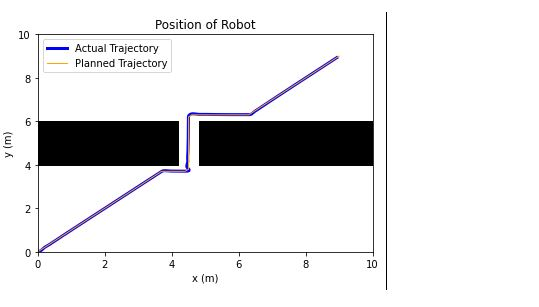
\includegraphics[width=18cm]{w3.JPG}
         \caption{Figure Showing path planning for world 3}
    \end{figure}
\end{center}

    The time for planning for world 4 was 6.37 seconds  and the trajectory is inserted below: \\ 
    \renewcommand{\thefigure}{5.1.4.4}
\begin{center}
    \begin{figure}[H]
        \centering
        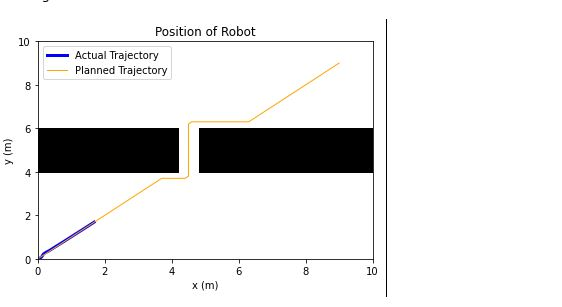
\includegraphics[width=18cm]{w4.JPG}
         \caption{Figure Showing path planning for world 4}
    \end{figure}
\end{center}

   The time for planning for the empty world  was 6.27 seconds  and the trajectory is inserted below: \\ 
    \renewcommand{\thefigure}{5.1.4.5}
\begin{center}
    \begin{figure}[H]
        \centering
        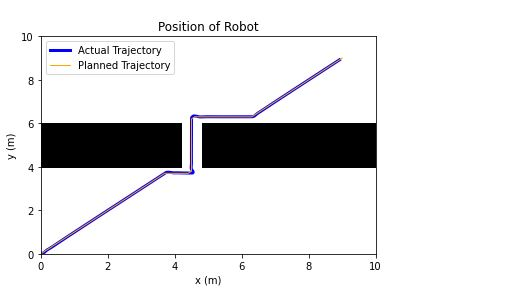
\includegraphics[width=18cm]{w5.JPG}
         \caption{Figure Showing path planning for empty world}
    \end{figure}
\end{center}


Clearly the A* planner works well where segments were calculated as straight line paths 
    
    \item Astar: A* would have an advantage because it's fast, and if there's a simple solution, A* can find it really easily and quickly. Some disadvantages would be how to find a good heuristic that incorporates all the joints. Also it would be hard to map out the 3D world and identify the obstacles and check for collision. It should also consider joint limits and the '8 connected' model might not work for all the joints. It's hard to work with a mix of R and P joints.
    
    RRT: The disadvantage would be it might take a very long time to come up with a solution. Also, it's possible that it can come up with a solution that's too complicated and has many small twists and turns. An advantage would be that if a joint moves in a weird/particular way, the algorithm can easily move accordingly. It can work with R and P joints and consider how each of them move separately.
    
    \item The software only succeeds sometimes. There are a lot of times where the trajectory is planned out, but the robot doesn't follow it or fails in the middle of following. 
    
    \item The difficult plans are ones where there are small and complicated turns. Sometimes especially RRT gives trajectory that makes small turns and twitches, and in those situations the robot would fail.
    
    \item The planned trajectory is not always the simulation result. Most of the times the robot follow the trajectory closely. However, there are times where the robot completely goes off the trajectory and fails. There are other times the robot skew away from the trajectory a little bit, but then goes back on the right track. There are times where the robot seems like it's following the trajectory well, but then stops in the middle. The error between these two varies dramatically.
    
    \item In a physical setting, the planner would work similarly. The input is the map of the setting, with the obstacles clearly labeled. This might be difficult in a dynamic situation or an unclear new environment. If the robot doesn't know the environment parameters, then the algorithm wouldn't be effective. As for the trajectory planning, the robot will face real world problems like slippery floor and hitting itself while turning. It also can't have dramatic turns that could cause it to topple. It should be careful to not go too fast as it might topple when changing directions.
    
    \item If we had more time, we would also write our own RRT algorithm just to practice! For the A* algorithm, one problem we have is that the step size is 0.5 right now, meaning each turn we check the 8 steps that are 0.5 away from it $(0, -0.5), (0, 0.5), (-0.5, 0), (0.5, 0), (-0.5, -0.5), (-0.5, 0.5), (0.5, -0.5), (0.5, 0.5))$. If there is a really narrow pathway that is less than 0.5 wide, the algorithm wouldn't be able to find it. If we had more time, we would implement something that can adjust the step size according to the size of map and radius of the robot. I would also add a maximum iteration field to it, in order to prevent situations where it take way too long to output a 'None' answer. An alternative is to add warnings that pop up so that the user know how much the algorithm has explored. I think the algorithm could be sped up through vectorizing some of the functions and removing unnecessary loops. Also, a good thing to do would be to write code to visualize the results and the map each time. 


\end{enumerate}
\newpage  




%%%%%%%%%%%%%% Making  a Great Figure %%%%%%%%%%%%%%%%%%
% \renewcommand{\thefigure}{1.2.1}
% \begin{center}
%     \begin{figure}[H]
%         \centering
%         \includegraphics[width=18cm]{diagram_ii.JPG}
%          \caption{Figure Showing T_5^0}
%     \end{figure}
% \end{center}


% \begin{figure}
%   \centering
%   \fbox{\rule[-.5cm]{4cm}{4cm} \rule[-.5cm]{4cm}{0cm}}
%   \caption{Sample figure caption.}
%   \label{fig:fig1}
% \end{figure}

% \subsection{Tables}
% \lipsum[12]
% See awesome Table~\ref{tab:table}.


% %%%%%%%%%%%%%%%% MAKING A  GOOD TABLE %%%%%%%%%%%%%%%%%
% \begin{table}
%  \caption{Sample table title}
%   \centering
%   \begin{tabular}{lll}
%     \toprule
%     \multicolumn{2}{c}{Part}                   \\
%     \cmidrule(r){1-2}
%     Name     & Description     & Size ($\mu$m) \\
%     \midrule
%     Dendrite & Input terminal  & $\sim$100     \\
%     Axon     & Output terminal & $\sim$10      \\
%     Soma     & Cell body       & up to $10^6$  \\
%     \bottomrule
%   \end{tabular}
%   \label{tab:table}
% \end{table}


%%%%%%%%%%%%% MAKING LISTS %%%%%%%%%%%%%%%%%%%%%%%%%%%
% \subsection{Lists}
% \begin{itemize}
% \item Lorem ipsum dolor sit amet
% \item consectetur adipiscing elit. 
% \item Aliquam dignissim blandit est, in dictum tortor gravida eget. In ac rutrum magna.
% \end{itemize}



%  \bibliographystyle{unsrt}  
%  \bibliography{references}  
 \newpage
 
 \section{Appendix}
%%%%%%PUT CODE HERE (CHANGE "PYTHON-CODE.py") %%%%%%%%%%%

\lstinputlisting[caption = mobile\_controller.py]{mobile_controller.py}
\pagebreak





 
\end{document}